\subsection{Wellenlängenselektion}

\subsubsection{Selektion über Reflektivität der Spiegel}

\paragraph{Aufbau und Durchführung}

bei gelber PI:
Messung mit kleinem power head
grün dabei bei kleinen Strömen


\paragraph{Auswertung}
blabla

\begin{figure}[H]
\begin{center}
  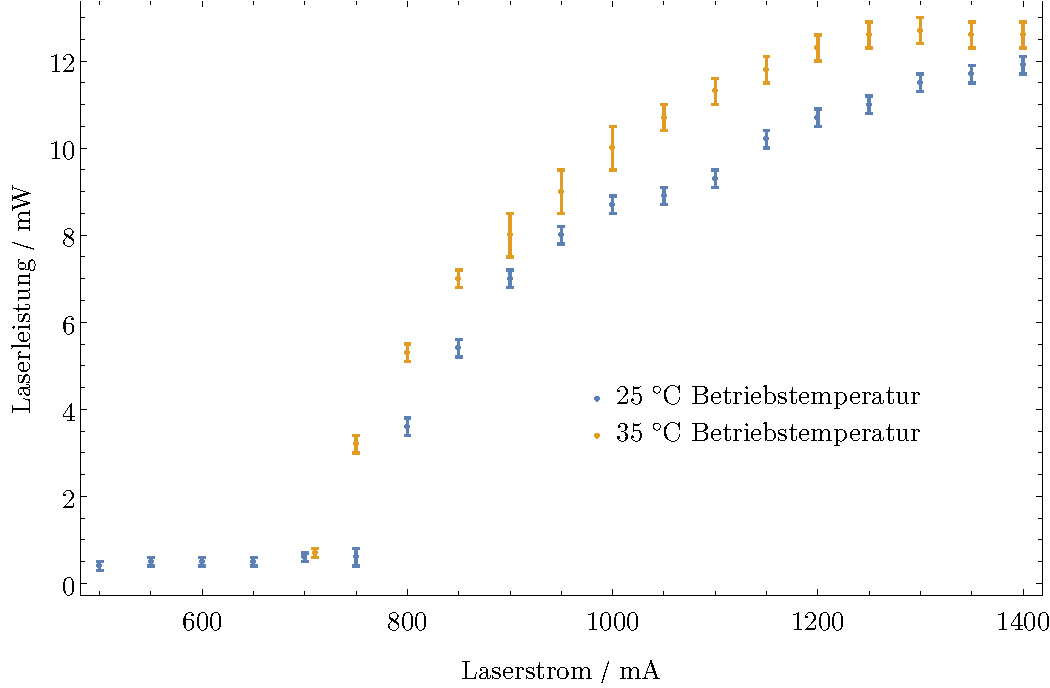
\includegraphics[width=\textwidth]{PI_gruen.pdf}
  \caption{PI-Kennlinie des grünen Lasers bei 25\grad und 35\grad
  Betriebstemperatur.}
  \label{img:PI_gruen}
\end{center}
\end{figure}


\begin{figure}[H]
\begin{center}
  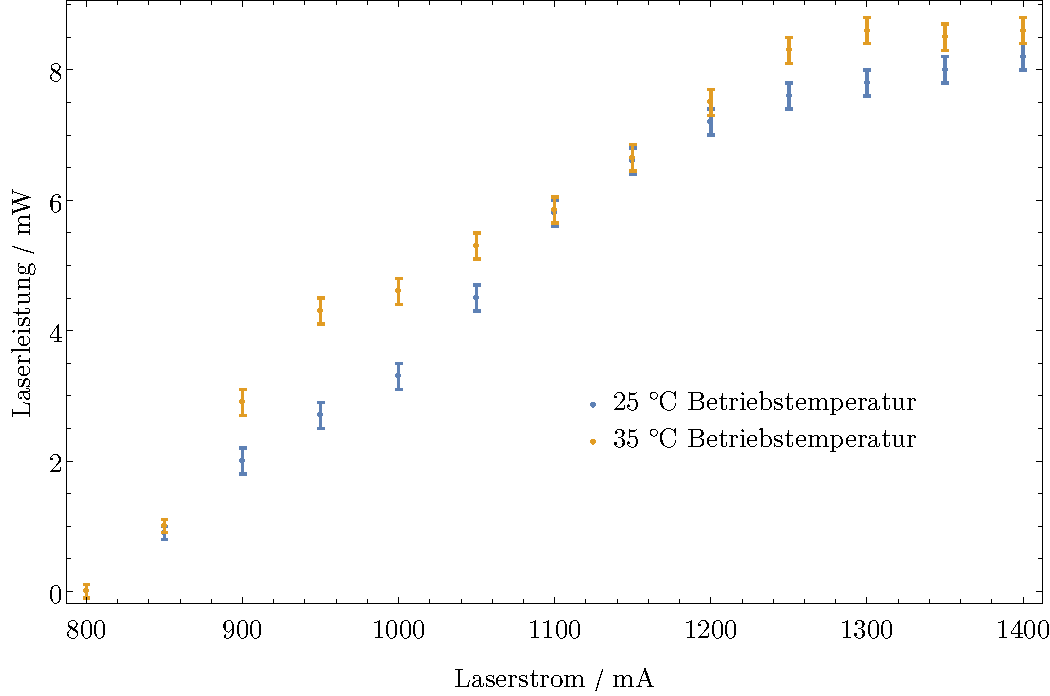
\includegraphics[width=\textwidth]{PI_gelb.pdf}
  \caption{PI-Kennlinie des gelben Lasers bei 25\grad und 35\grad
  Betriebstemperatur.}
  \label{img:PI_gelb}
\end{center}
\end{figure}



\subsubsection{Selektion über doppelbrechenden Kristall}


\paragraph{Aufbau und Durchführung}
blabla

\paragraph{Auswertung}
blabla

\begin{figure}[H]
\begin{center}
  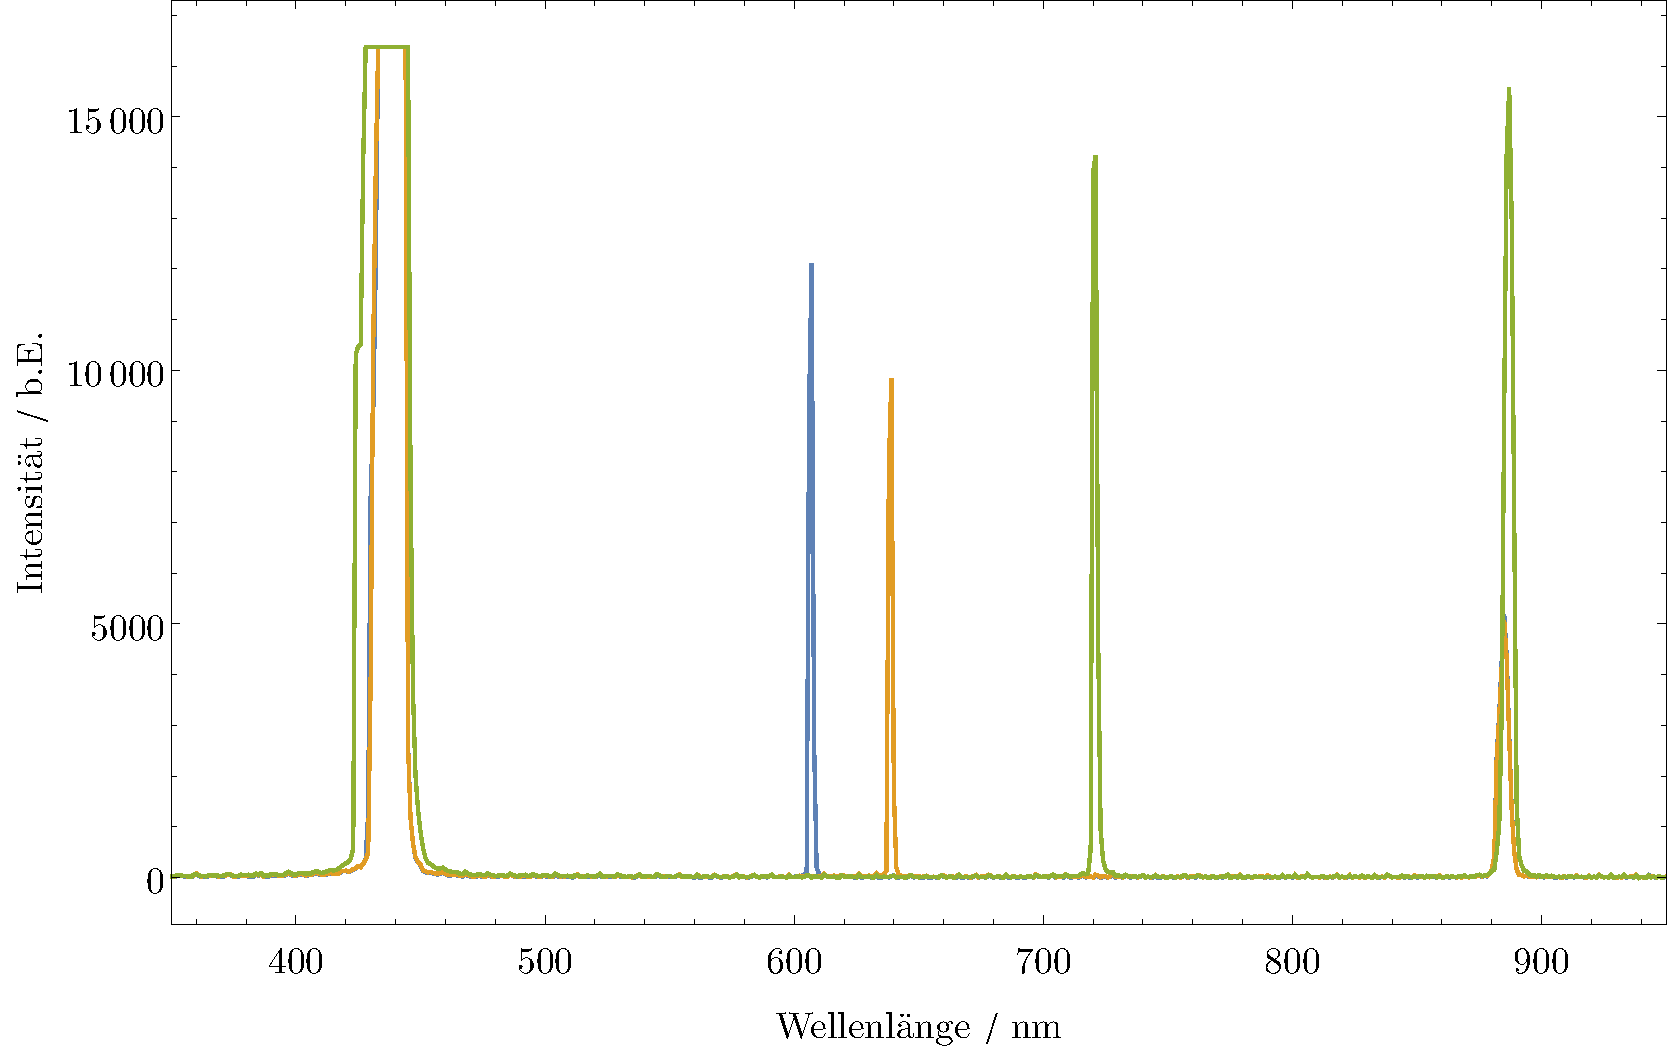
\includegraphics[width=\textwidth]{BifrSpekt.pdf}
  \caption{Spektren des Lasers für drei unterschiedliche Winkel des doppelbrechenden Kristalls.}
  \label{img:BifrSpekt}
\end{center}
\end{figure}

\subsubsection{Selektion mit Littrow-Prisma}

\paragraph{Aufbau und Durchführung}
blabla


\paragraph{Auswertung}

%an ab 0°
%max: 20°, dann stärker und schwächer
%aus ab 80°
%an bei 180°
%max: 200° wird stärker und schwächer bis 260°, hört auf, fängt an bei 0°

%dunkelrote linie
%an ab 270° bis 0°
%max: 315°
%an ab 80° bis 170°
%max bei 110°

\begin{figure}[H]
\begin{center}
  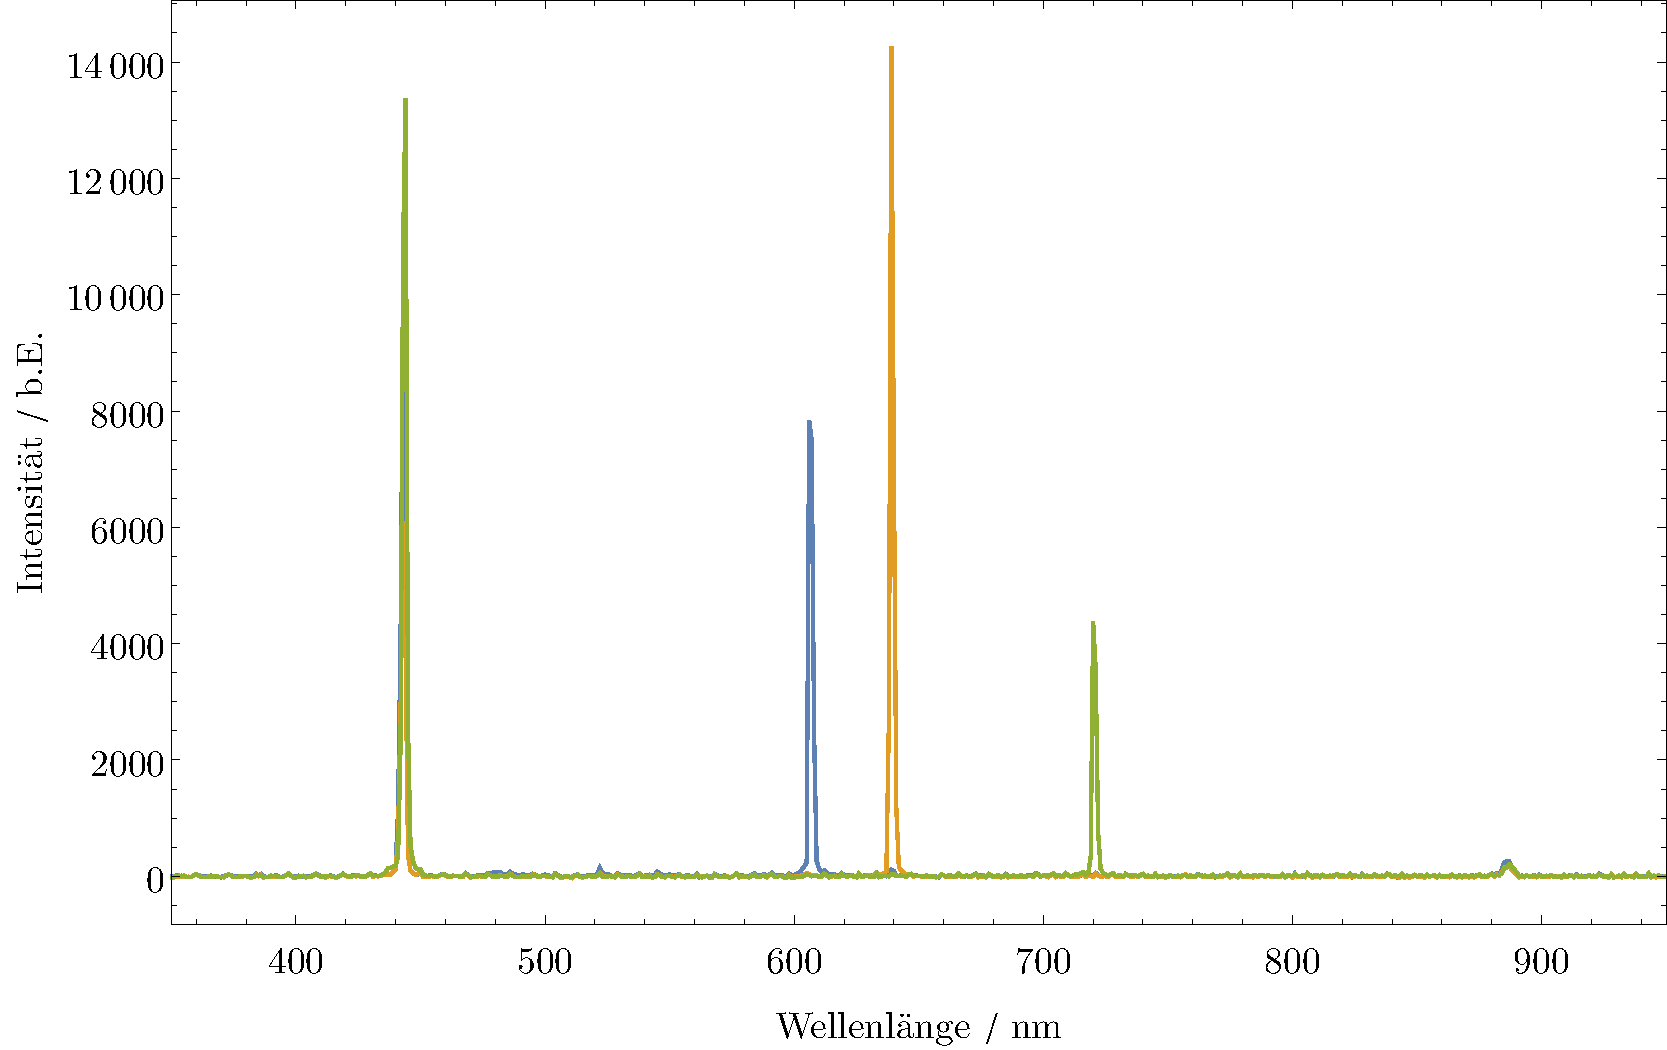
\includegraphics[width=\textwidth]{LittrSpekt.pdf}
  \caption{Spektren des Lasers für drei unterschiedliche Einstellungen des Littrow-Prismas.}
  \label{img:LittrSpekt}
\end{center}
\end{figure}
